\chapter{The Daya Bay Reactor Antineutrino Experiment}
\label{ch:detector}

The Daya Bay Reactor Antineutrino Experiment was designed
to be sensitive to $\thetaot \sim 0.01$
by performing a relative measurement of the rate of \nuebar{}
using a modular detector system arranged at near and far sites \cite{dybproposal2006}.
The experiment is located in southeast China,
approximately \SI{55}{\km} northeast of Hong Kong,
on the campus of the Daya Bay and Ling Ao Nuclear Power Plants.
Groundbreaking for civil construction of the three underground
experimental halls occurred in October 2007,
and construction lasted approximately 4 years \cite{dyb_overview}.
The antineutrino detectors in the first experimental hall (EH1)
were ready for data taking on 11 August 2011,
and EH2 was ready on 5 November 2011.
With the completion of EH3, data taking began on 24 December 2011
and, with only brief interruptions,
continued until 12 December 2020.

The Daya Bay site is ideal for an oscillation experiment.
Its six reactor cores together form one of the most intense \nuebar{}
sources on Earth \cite{detector_system}.
The power plant campus is also located at the base of a mountain ridge,
providing an ideal location for antineutrino detectors that must be
protected from cosmic-ray muons without having to dig deep mines.
The tunnel layout allows for easy access to the experiment via electric golf cart.

\section{Reactors and experimental halls}

Six pressurized-water nuclear reactors are used
as the \nuebar{} source for Daya Bay.
Each reactor has an output of \SI{2.9}{\giga\watt_{th}}
and combined they produce approximately \num{3.5e21}\,\nuebar/s \cite{ngd2016}.
The reactors are arranged in three pairs: Daya Bay, Ling Ao, and Ling Ao II.
The location of the cores determined the layout of the Daya Bay experiment.

The experiment is arranged into three experimental halls (EHs).
EH1 is located close to the Daya Bay cores (\SIrange{357}{372}{\meter}),
and EH2 is located close to the Ling Ao and Ling Ao II cores
(\SIrange{467}{558}{\meter}).
They are therefore known collectively as the near halls.
Their purpose is to constrain the \nuebar{} flux for the
relative oscillation measurement,
and they each contain two antineutrino detector modules (ADs).
EH3 is located farther away, approximately \SI{2}{\km} from the Daya Bay cores
and \SI{1.5}{\km} from the Ling Ao cores,
and is correspondingly called the far hall.
EH3 is located at the first oscillation minimum
for the oscillation controlled by $\Delta m^2_{32}$ (and $\Delta m^2_{31}$)
and its purpose is to measure the decrease in \nuebar{} rate compared to the near halls.
To increase statistics, EH3 contains four ADs.
The layout of the EHs with respect to the reactors is shown in \cref{fig:layout}.

\begin{figure}
    \centering
    \begin{subfigure}{0.49\textwidth}
        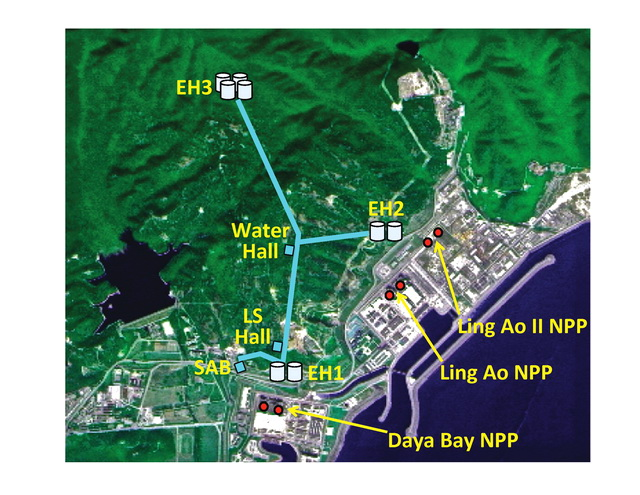
\includegraphics[width=\textwidth]{ch_detector/dayabay_map}
    \end{subfigure}
    \begin{subfigure}{0.49\textwidth}
        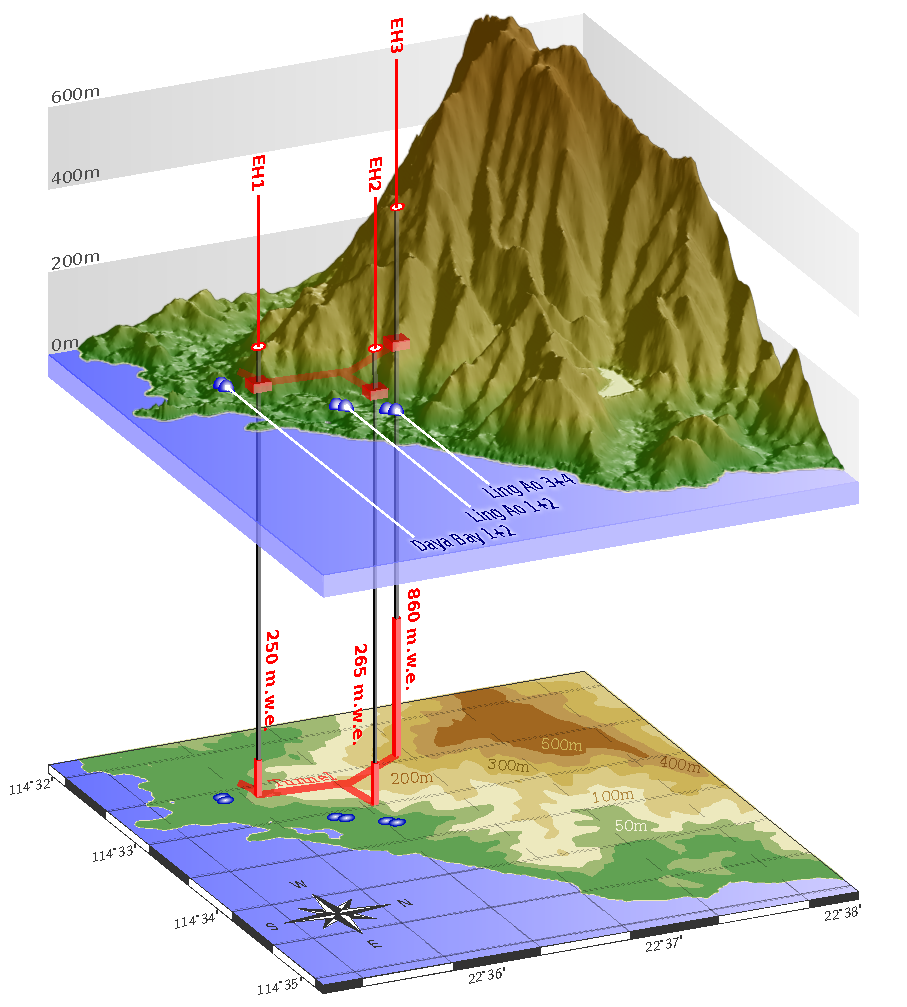
\includegraphics[width=\textwidth]{ch_detector/dayabay_map_3d}
    \end{subfigure}
    \caption{Two views of the layout of the Daya Bay experiment.}
    \label{fig:layout}
\end{figure}

The EHs are located at underneath a mountain, which provides a substantial
overburden to protect against cosmic-ray muons.
The specific measurements of overburden, the positions of the ADs,
%and the baseline are shown in \cref{tab:baselines}.

%\begin{table}[ht]
    %\centering
    %\begin{tabular}[t]{lSSSSSSSSSSSS}
        %\toprule
        %\midrule
        %\bottomrule
    %\end{tabular}
    %\caption{Baselines and overburdens}
    %\label{tab:baselines}
%\end{table}

To accelerate the experiment startup timeline,
only six of the planned eight ADs were installed in 2011:
2 in EH1, 1 in EH2, and 3 in EH3.
This so-called 6-AD period lasted from 24 December 2011 until 28 July 2012. % Put exact dates
The experiment was shut down while the remaining two ADs were installed
in EH2 and EH3.
The 8-AD period began on 19 October 2012.
At the end of 2017, EH1-AD1 was chosen to be repurposed as a test stand
for liquid scintillator studies for the JUNO experiment \cite{junoproposal2016},
and was decommissioned from Daya Bay.
The 7-AD period began in January 2017 and continued through the end of
the Daya Bay experiment on 12 December 2020.

The ADs within each hall are collectively surrounded by a water pool,
which acts as a passive shield against natural radioactivity present in the rock
as well as an active veto for muons which penetrate through the overburden.
The water pool is covered by a resistive plate chamber (RPC) array
to provide additional sensitivity to incoming muons.
\Cref{fig:eh3_wp_photo} shows a photograph of EH3 during installation of the ADs,
when the RPC had not yet been moved into position to cover the water pool.
Also visible mounted to the near and far walls are two muon RPC telescopes
which were used for muon studies during detector commissioning \cite{muonsystem2015}.

\begin{figure}
    \centering
    \includegraphics[width=0.5\textwidth]{ch_detector/EH3_installation_6ADperiod}
    \caption{EH3 during the installation of the first three ADs.}
    \label{fig:eh3_wp_photo}
\end{figure}

\section{Antineutrino detectors}

The eight antineutrino detectors (ADs) are used to measure
the rate and energy of millions of \nuebar{} interactions with high precision
and low systematic uncertainty.
Each AD consists of three concentric cylindrical regions
contained in an outer stainless steel vessel (SSV),
a cylinder with diameter and height of \SI{5}{\m}.
The innermost region is filled with \SI{0.1}{\percent} by mass
Gadolinium-doped liquid scintillator (GdLS).
The GdLS is contained within an acrylic cylinder known as the inner acrylic vessel (IAV).
The middle region between the IAV and the outer acrylic vessel (OAV) is filled
with (plain, undoped) liquid scintillator (LS).
The outer region between the OAV and SSV is filled with mineral oil
that serves as a final passive layer of shielding around the LS region.

Two views of the nested AD configuration are shown in \cref{fig:ad_cutaway}.
The IAV has a height and diameter of \SI{3}{\m} and is filled with \SI{20}{\tonne}
of GdLS.
The OAV has a height and diameter of \SI{4}{\m} and is filled with \SI{20}{\tonne}
of LS.
The SSV has a height and diameter of \SI{5}{\m} and is filled with \SI{40}{\tonne}
of mineral oil.
Each acrylic vessel is made of UV-transparent acrylic
and has a thickness of approximately \SI{1.5}{\cm}.

The liquid scintillator cocktail was designed to optimize the optical properties
and maximize stability over time \cite{gdls2014}.
Linear alkylbenzene (LAB) is used as the solvent and \nuebar{} target,
into which \SI{3}{\g\per\liter} of 2,5-diphenyloxazole (PPO)
is dissolved as a fluor,
along with \SI{15}{\mg\per\liter} of the wavelength shifter
p-bis-(o-methylstyryl)-benzene (bis-MSB).
This LS is used to fill the OAV.
To dissolve Gd into the LS to fill the IAV, the chelating ligand
3,5,5-trimethylhexanoic acid (TMHA) was chosen for its ease of production
and its stability in solution with LAB.
During LS production, the approximately \SI{185}{\tonne} of GdLS for the IAV
was produced first,
after which the equipment was cleaned with a diluted HCl solution and purified water
so that the undoped LS could then be produced for the OAV.

Each AD contained overflow tanks to allow the liquid in each region
to respond to the slight expected changes in temperature and pressure.
ADs were also fitted with three automated calibration units (ACUs)
which contained radioactive sources and LEDs to help calibrate the ADs.
The ACUs are described in detail in \cref{ch:calibration}.

The mineral oil region also contained the 192 8-inch Hamamatsu R5912
photomultiplier tubes (PMTs) that monitored the AD for scintillation light
(and, secondarily, Cherenkov radiation).
The PMTs are arranged in 8 rings of 24 PMTs on the outer edge of the mineral oil region.
Light collection and detector uniformity is increased by the presence of
specular reflectors located on the top and bottom faces of the OAV,
as indicated in \cref{fig:ad_cutaway}.
PMTs consist of a sensitive photocathode, from which an incident photon
can eject an electron by the photoelectric effect.
The photoelectron (PE) is accelerated in an electric field to the first dynode,
a charged metal plate, where it causes multiple electrons to be ejected.
A series of subsequent dynodes leads to an avalanche effect of electrons,
which are collected at the anode and read out as a voltage signal.
When discussing the strength of a PMT signal,
it is customary to use the term ``charge'' (measured in photoelectrons)
rather than ``light,''
though the charge collected by a PMT anode
is of course a proxy for the number of incident photons.

Before the ADs were filled with LS, GdLS, and mineral oil,
they were tested in a series of so-called dry runs \cite{dryrun1}.
The PMTs were supplied with high voltage
to verify the stability of the gain and dark rate.
The ACUs were deployed, and the calibration LEDs
were used to induce charge signals on the PMTs
to exercise not only the PMTs but also the front-end electronics,
the online DAQ system and the offline storage.
It was during the dry runs that the issue of PMT light emission,
or flasher events, was discovered.
These events must be filtered out from the data stream,
as described in \cref{sec:flashers}.

\begin{figure}
    \centering
    \begin{subfigure}{\textwidth}
        \centering
        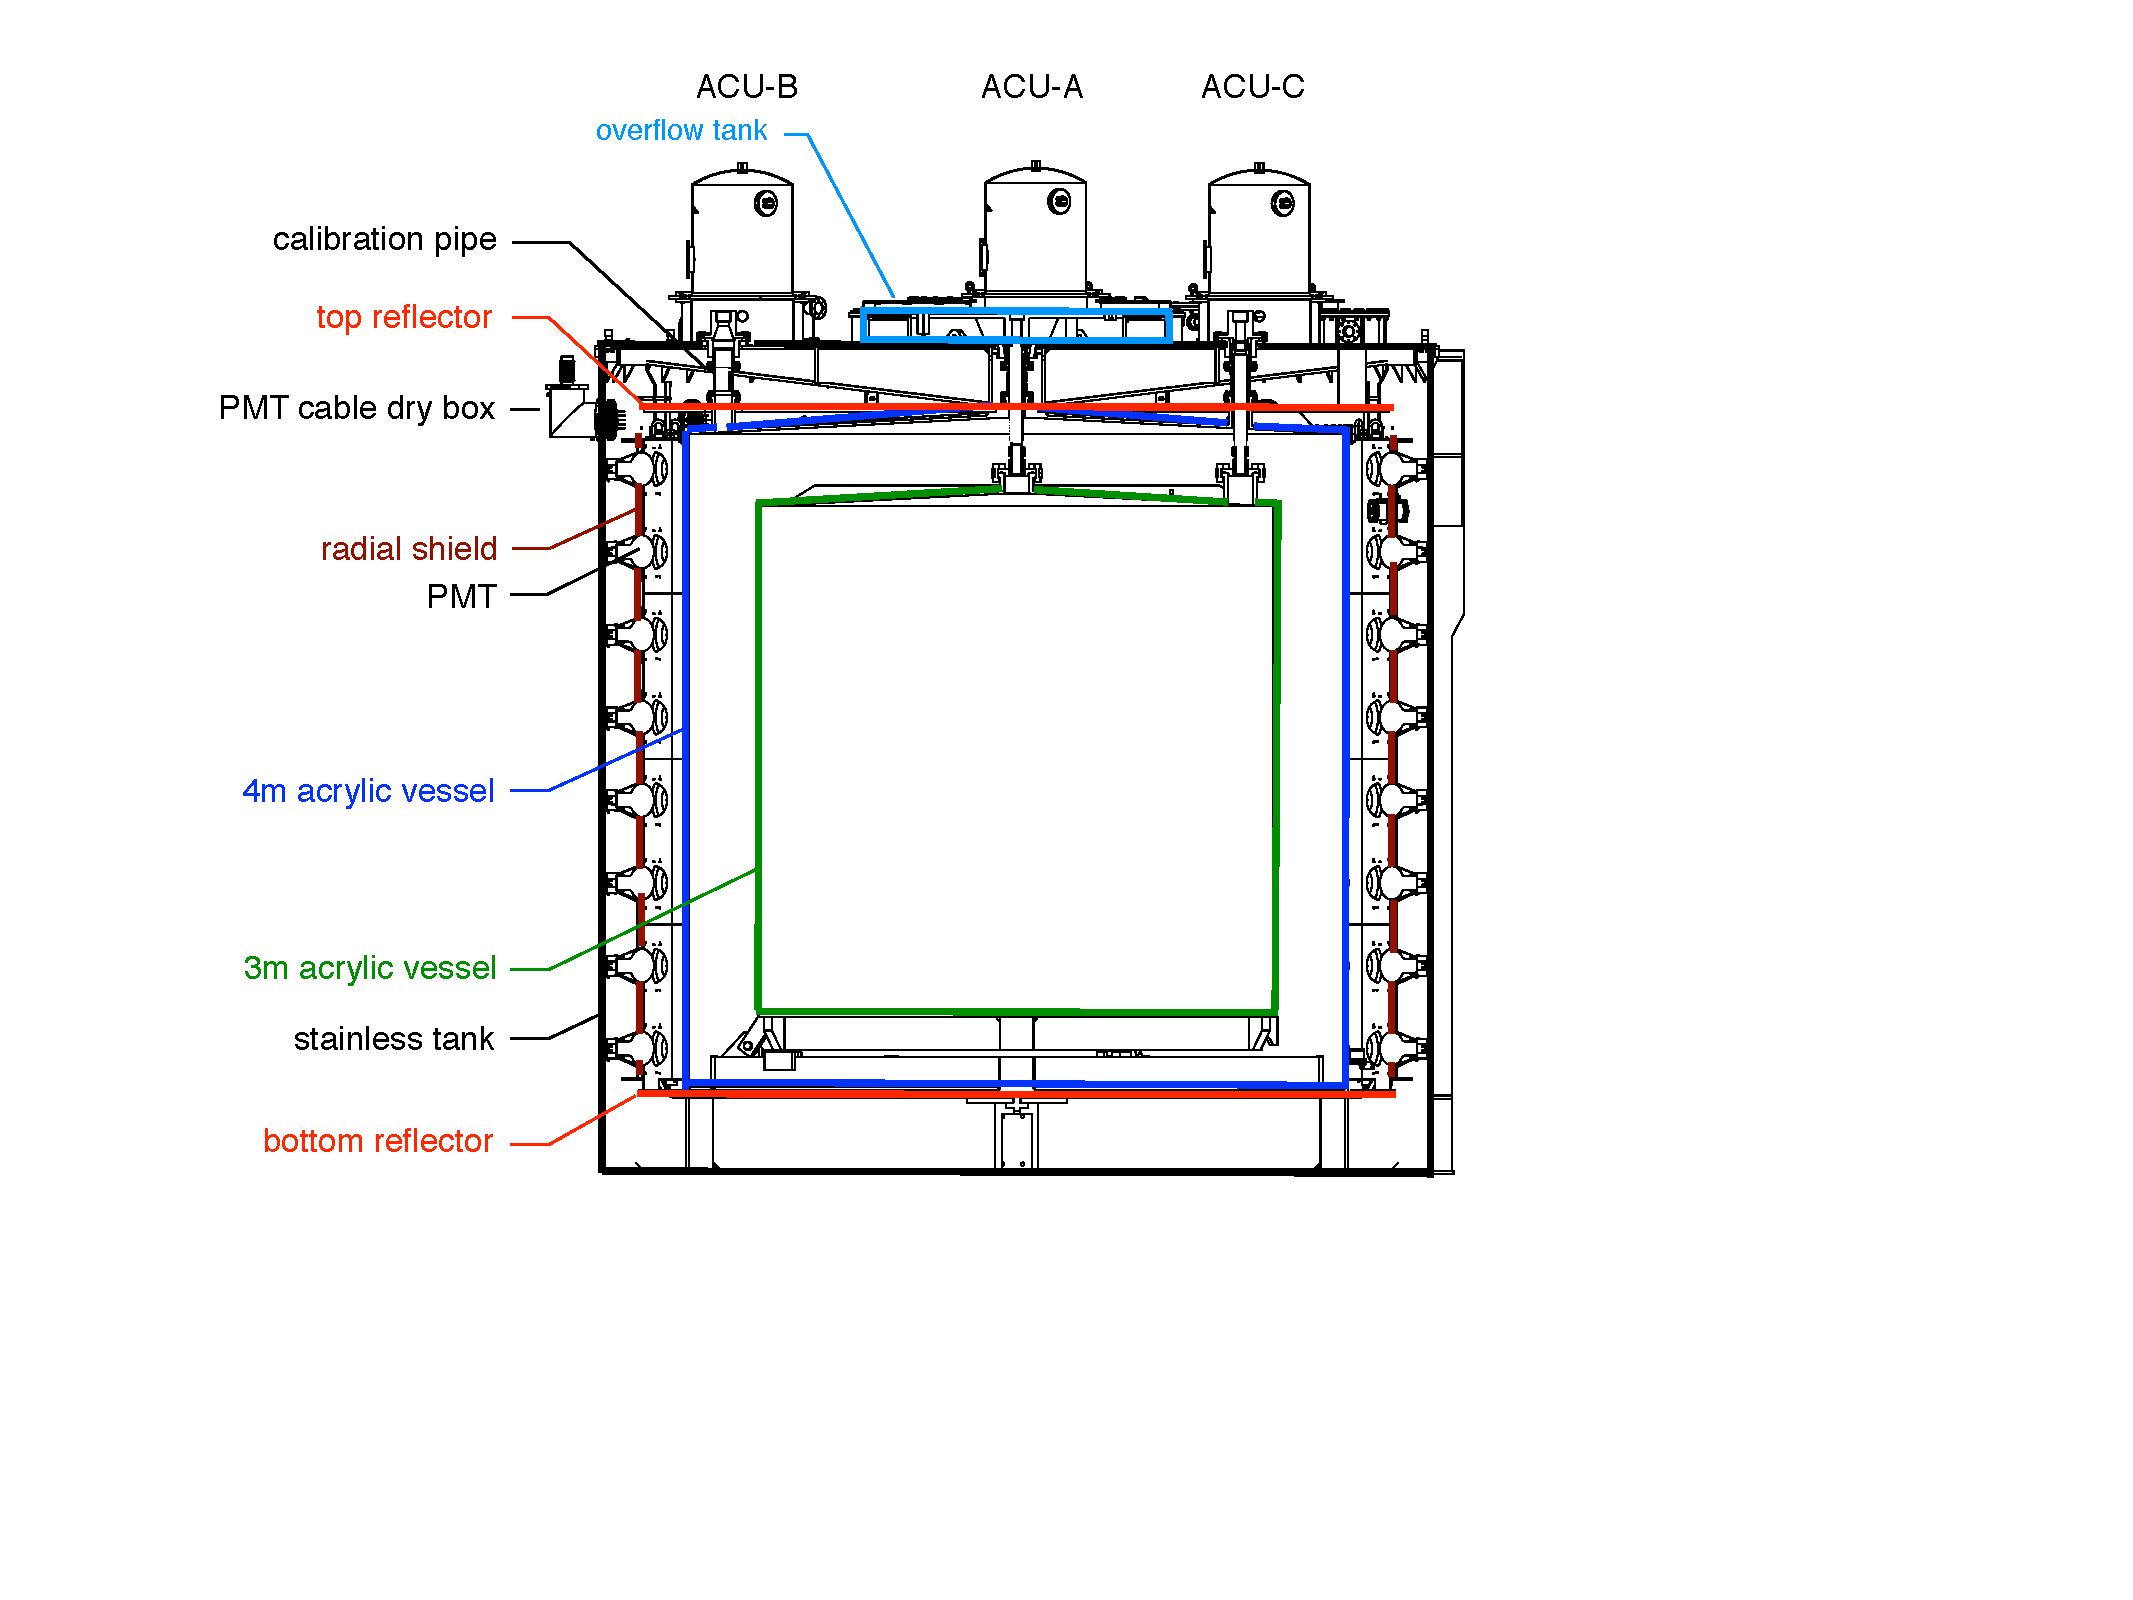
\includegraphics[height=0.4\textheight]{ch_detector/ADcutaway_2D}
    \end{subfigure}
    \vspace{1cm}\\
    \begin{subfigure}[0.4\textheight]{\textwidth}
        \centering
        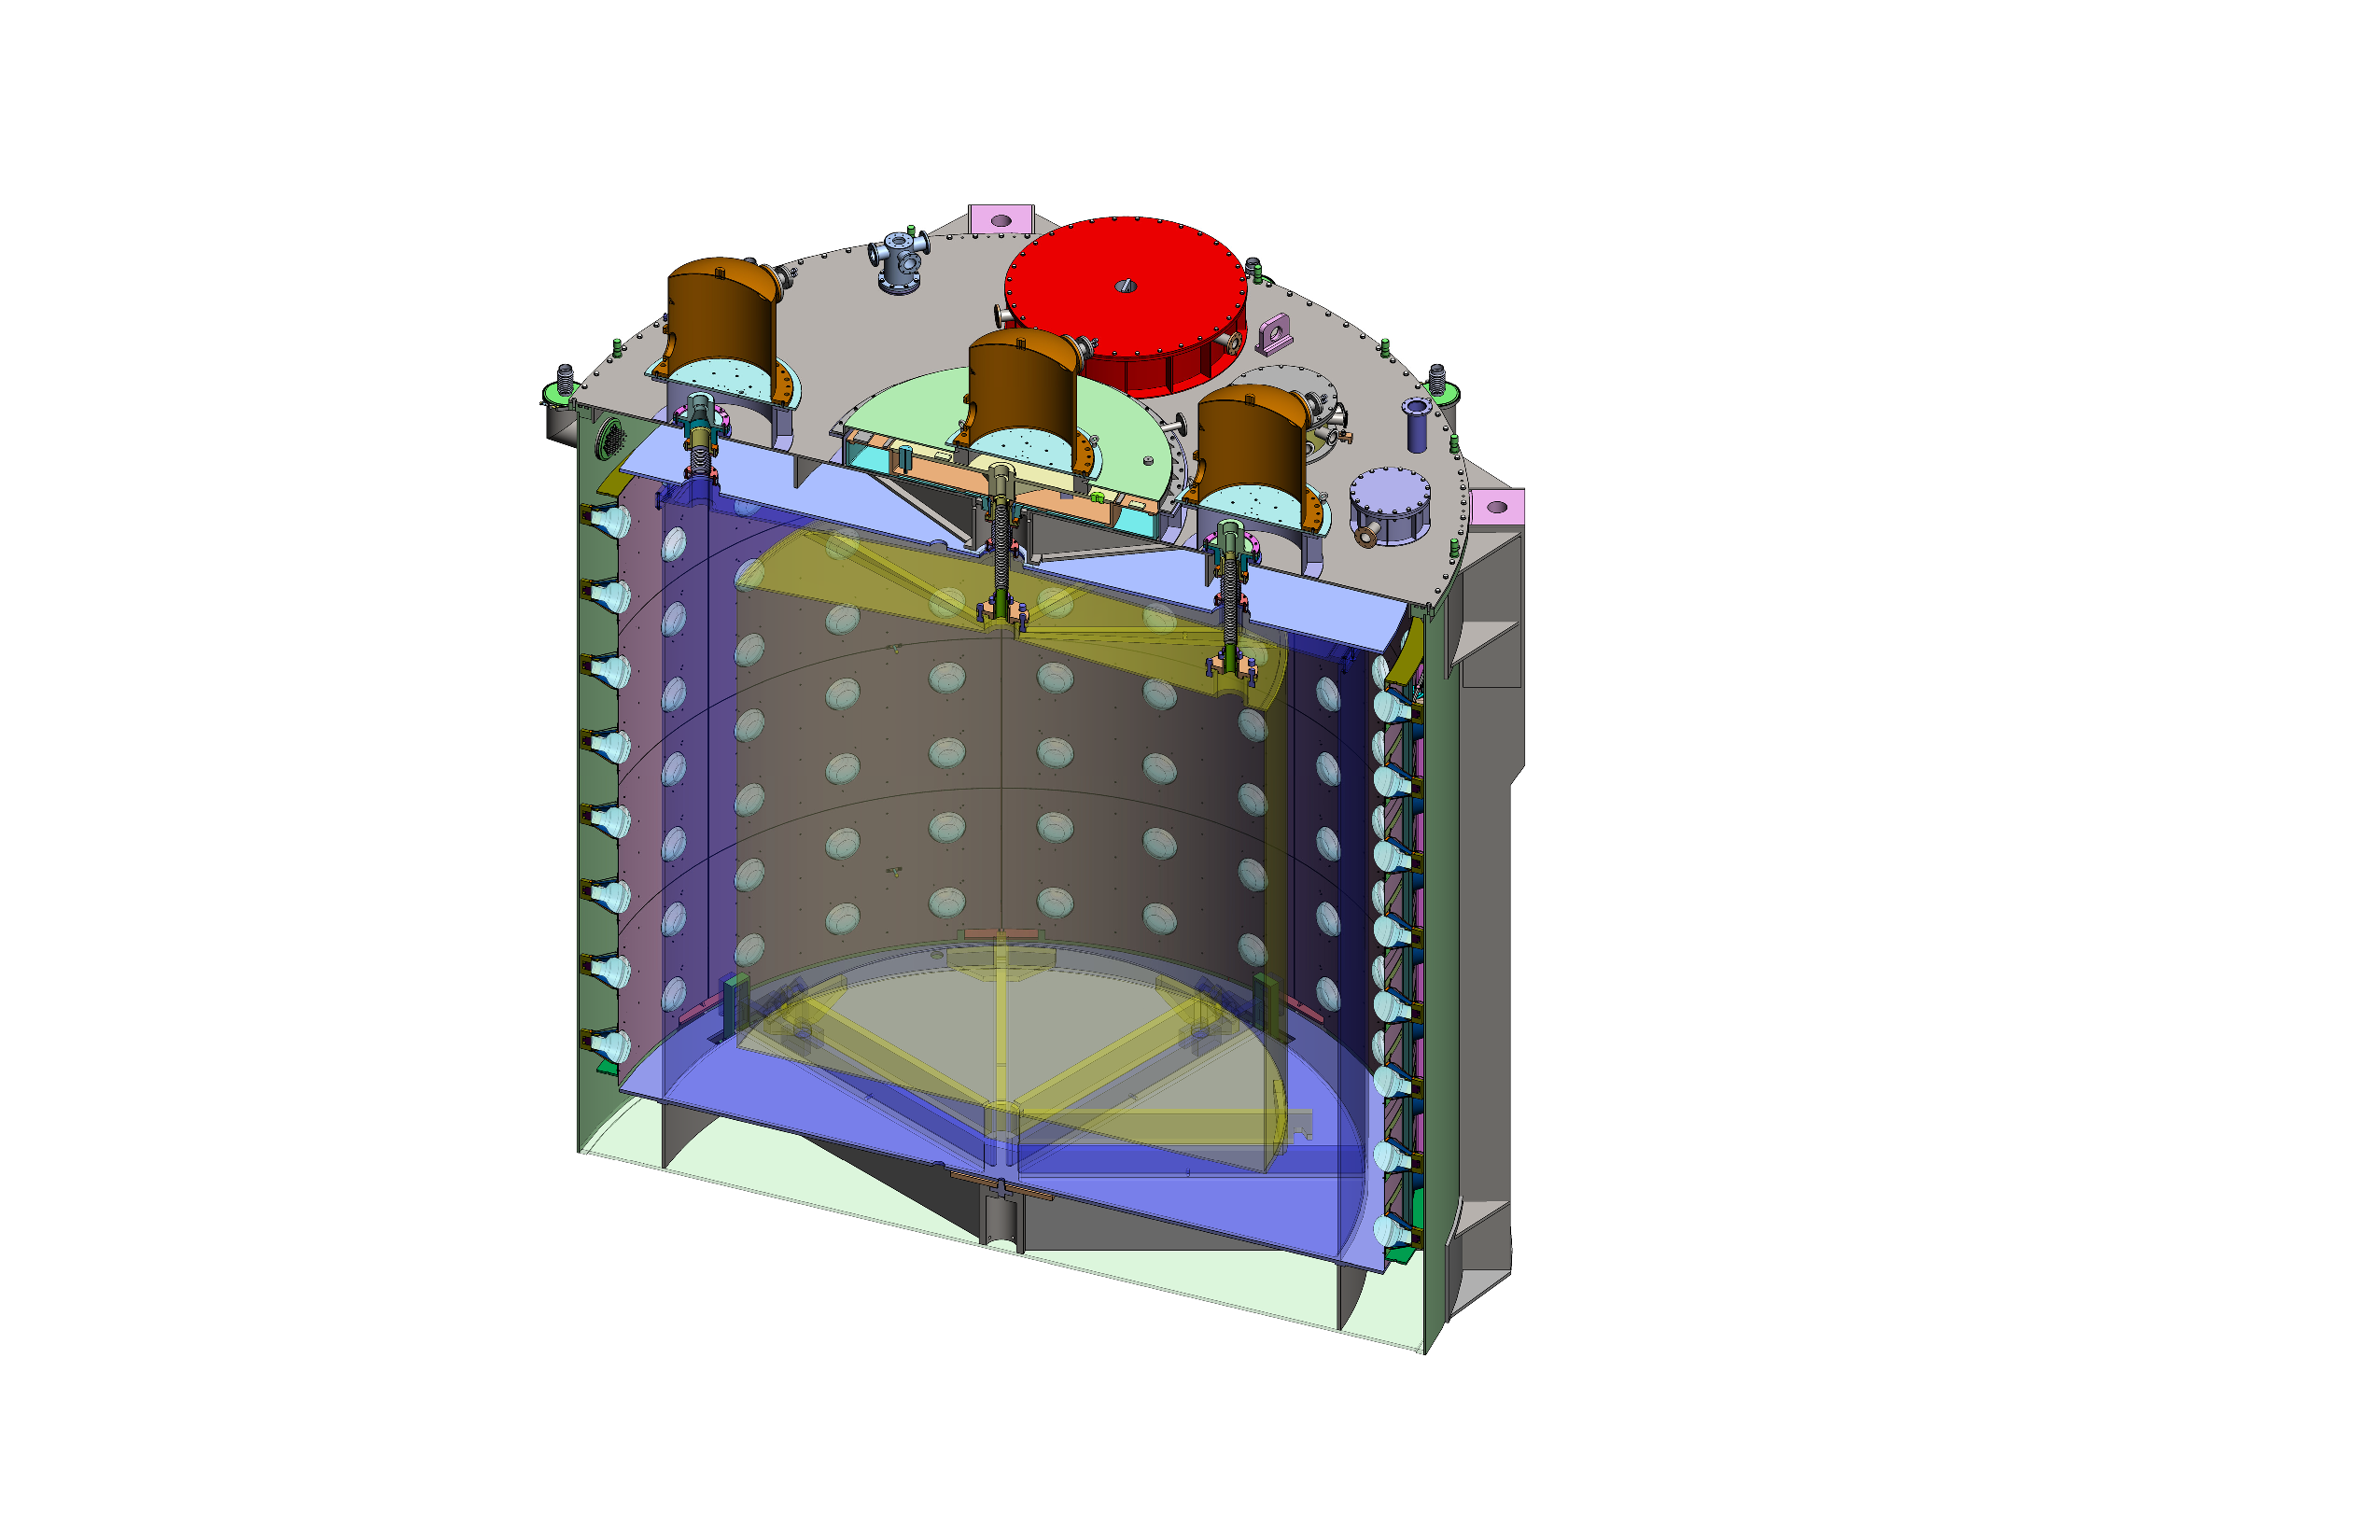
\includegraphics[height=0.4\textheight]{ch_detector/ADcutaway}
    \end{subfigure}
    \caption{
        Two views of the Daya Bay antineutrino detector (AD) \cite{ngd2016}.
        The coordinate system origin is in the center of the GdLS region,
        as indicated by the star symbol in the 2D view.
        Positive $z$ is upwards.
        \todo[inline]{Lower figure is from unused files in long paper SVN. Where to cite?}
    }
    % Use 2D figure from NIMA 811 (2016) 133
    \label{fig:ad_cutaway}
\end{figure}

\subsection{Observing Inverse Beta Decay}
\label{subsec:ibd_intro}

The IBD reaction, $\nuebar + p \to e^+ + n$,
creates two signals with a characteristic
time delay between them, in a pattern known as a ``double''
or ``delayed'' coincidence.
When this reaction occurred in either the GdLS or LS region
of a Daya Bay AD,
the positron quickly deposited its kinetic energy in the liquid scintillator
and annihilated within $\lesssim\SI{1}{\nano\second}$
into two \SI{0.511}{\MeV} $\gamma$-rays
which also deposited their energy into the LS.
The combined light from the kinetic energy and annihilation $\gamma$-rays
was the prompt signal
and served as an effective timestamp for the interaction.
The total prompt energy was related to the incident antineutrino energy
via the mass-energy conservation relation
\begin{equation}\label{eq:prompt_vs_nu_energy}
    E_p \approx E_\nu - \delta m_{pn} + m_e \approx E_\nu - \SI{0.78}{\MeV},
\end{equation}
where $\delta m_{pn}$ is the mass difference between the neutron and proton.
Meanwhile, the neutron produced by IBD thermalized in the liquid scintillator
and captured on Gd (in the GdLS only) or on a proton in the form of \isotope[1]{H}
(in both the GdLS and LS).
This happened with a characteristic time of $\sim \SI{28}{\micro\second}$
in GdLS and $\sim \SI{215}{\micro\second}$ in LS.
The shorter time in the GdLS was by design,
due to the large capture cross section of a thermalized neutron
on a Gd nucleus compared to H (\SI{49}{\kilo\barn} vs. \SI{0.332}{\barn})
\cite{gdls2014}.
The term nGd is used to refer to the process neutron capture on Gd
and the analysis of the data set containing nGd captures.
The analogue for neutron capture on H is nH.
For nGd captures, the excited nucleus
emitted $\gamma$-rays in one of two decay chains,
both of which had a combined energy of approximately \SI{8}{\MeV}.
The nH capture reaction $n+\isotope[1]{H} \to \isotope[2]{H} + \gamma$
would produce a \SI{2.2}{\MeV} $\gamma$-ray.
In either event, the $\gamma$-rays deposited their energy
in the liquid scintillator.
The \SIlist[list-pair-separator = { or }]{8;2.2}{\MeV} signal
from the neutron capture on Gd or H, respectively, comprised the delayed signal of the
double coincidence.
This prompt-delayed coincidence pattern was an extremely efficient
discriminator for IBD events against a wide variety of sources of background.
The full IBD interaction and detection process
is depicted in \cref{fig:ibd_cartoon}.

\begin{figure}
    \centering
    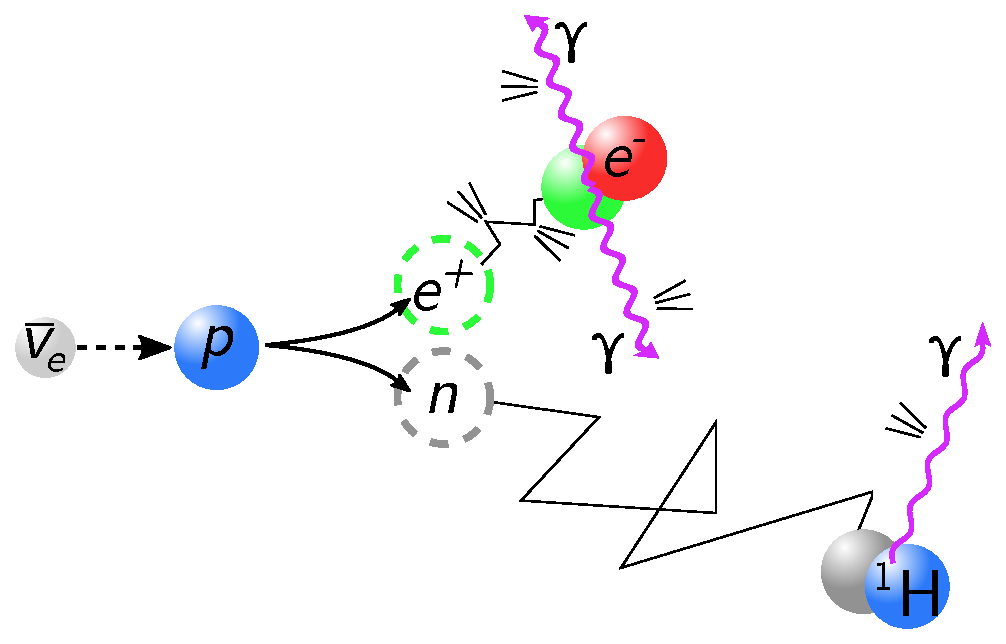
\includegraphics[width=0.8\textwidth]{ch_detector/ibd}
    \caption{
        Graphical depiction of the IBD interaction and delayed coincidence
        for neutron capture on hydrogen (nH).
        The dotted outlined $e^+$ and $n$ represent the initial interaction products.
        The thin black lines represent their trajectories
        through the liquid scintillator.
        The ``whisker'' marks indicate production of scintillation light.
    }
    \label{fig:ibd_cartoon}
\end{figure}

The LS region serves an important purpose for the main \thetaot{}
analysis using neutron capture on Gadolinium (nGd).
It significantly reduces the fraction of $\gamma$-rays from the nGd capture
that escape from the scintillating volume and distort the energy spectrum.
The presence of the LS region allows the entire GdLS volume to be
the fiducial volume, obviating the need to cut on the reconstructed position
of events, which would have added additional uncertainties to the analysis.
However, for the neutron capture on hydrogen analysis (nH),
the $\gamma$-rays produced by nH capture in the LS region
have a higher likelihood of escaping.
This risk is somewhat mitigated by the lower energy of the nH $\gamma$'s
(\SI{2.2}{\mev} vs. \SI{8}{\mev}).
The \thetaot{} analysis accounts for escaping $\gamma$'s
through assessment of the delayed energy cut efficiency (\cref{subsec:delayed}).


\section{Water pools and muon detectors}
\label{sec:wp}

The muon detection system for Daya Bay consists of
the water pool and the RPC system covering the water pool.
As data from the RPC is not used in the \thetaot{} analysis,
its description, along with extensive details of the entire muon system,
will be left to \cite{muonsystem2015}.
All three water pools are \SI{10}{\m} deep.
The near-hall water pools are \SI{10}{\m} wide and \SI{16}{\m} long,
while the far-hall water pool is \SI{16}{\m} in both dimensions.
These dimensions allow the water pools to provide at least \SI{2.5}{\m} of shielding
to the ADs in every direction.
A cutaway diagram of the near-site water pools is shown in \cref{fig:wpcutout}.
The water pool is divided using Tyvek(R) sheets
into optically-isolated inner and outer regions,
known as the inner water shield (IWS) and outer water shield (OWS).
Both the inner and outer water shields are instrumented with photomultiplier tubes (PMTs)
to detect the Cherenkov radiation from muons traversing the water.
The near-hall water pools each contain \num{288} PMTs,
and the far-hall water pool contains \num{384} PMTs.
A further breakdown is shown in \cref{tab:wp_pmts}.
\num{619} of these PMTs were newly-purchased \SI{20}{\cm}
model R5912 from Hamamatsu,
and the remaining \num{341} were \SI{8}{\inch} models 9350KA
and D642KB from EMI
donated by the MACRO experiment.
The IWS has been demonstrated to tag \SI{100}{\percent} of muons
that reach the ADs using the trigger thresholds described in \cref{tab:trigger}.


\begin{table}[ht]
    \centering
    \begin{tabular}[t]{llll}
        \toprule
        Hall & IWS & OWS (inward/outward) & Total\\
        \midrule
        EH1 & 121 & 167 (103/64) & 288\\
        EH2 & 121 & 167 (103/64) & 288\\
        EH3 & 160 & 224 (128/96) & 384\\
        \bottomrule
    \end{tabular}
    \caption{Muon system PMTs \cite{muonsystem2015}}
    \label{tab:wp_pmts}
\end{table}

\begin{figure}
    \centering
    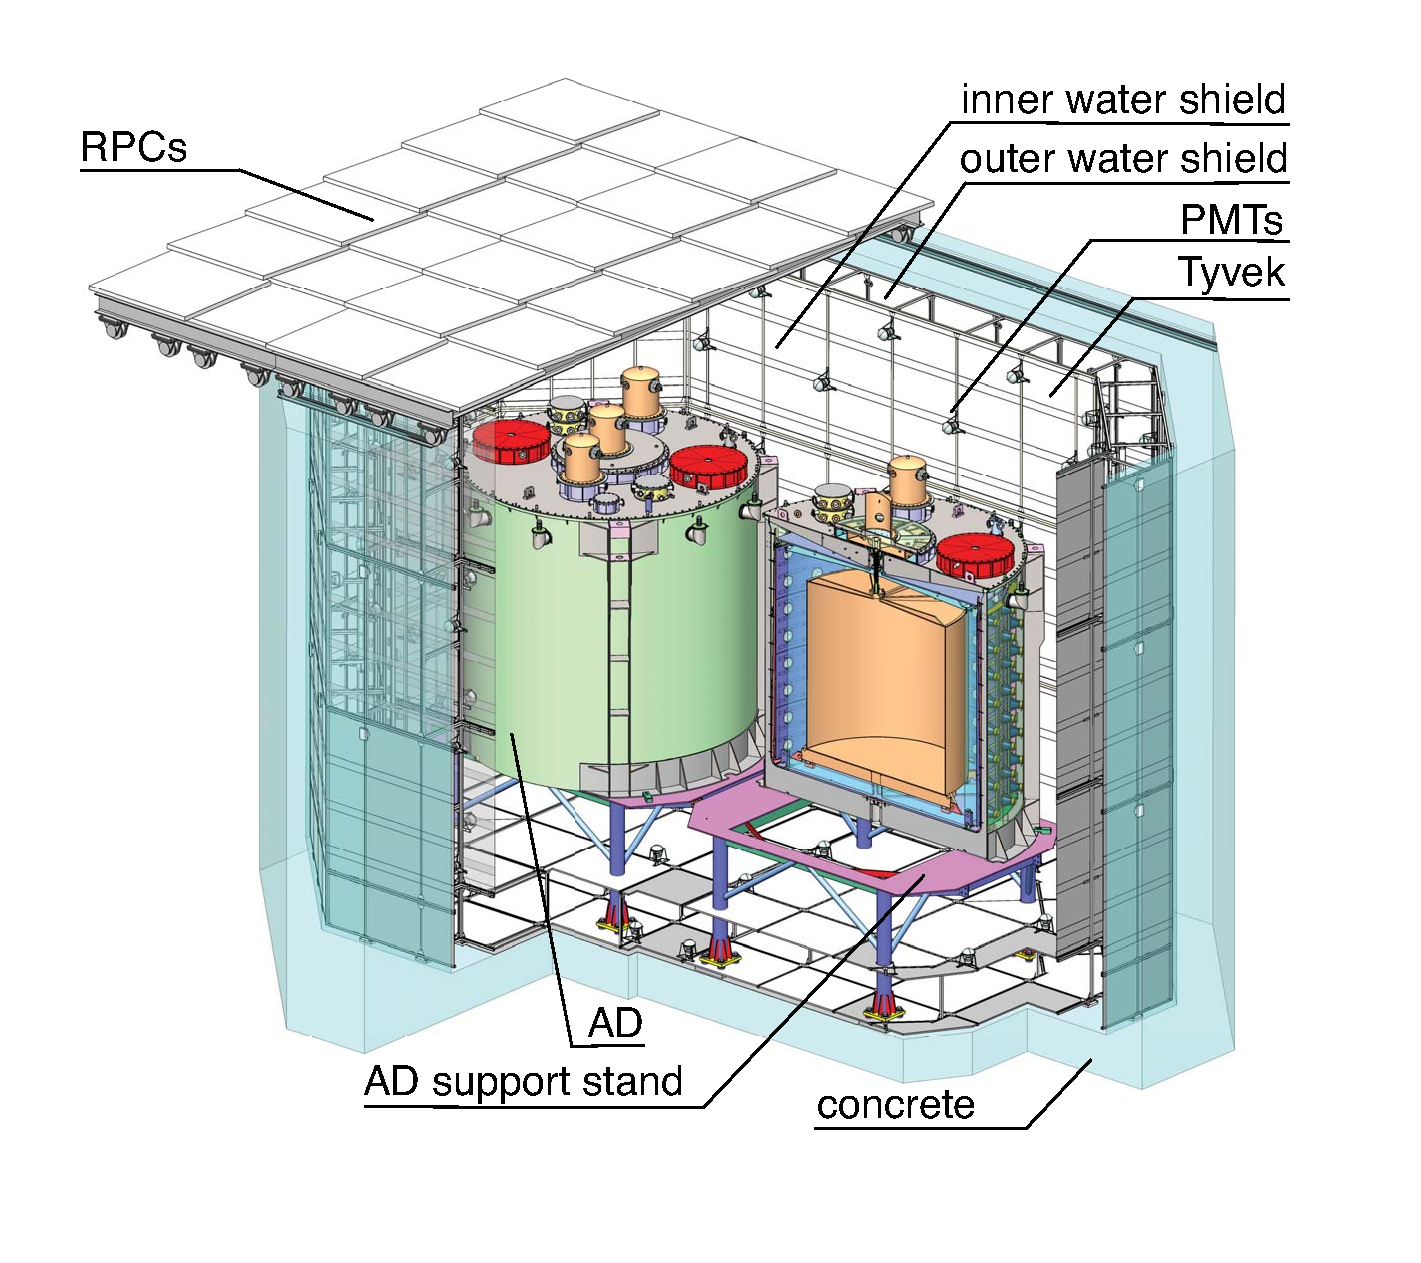
\includegraphics[height=0.4\textheight]{ch_detector/nearSiteDiagram}
    \caption{
        The water pool and AD layout in the near halls EH1 and EH2
        \cite{sidebyside}.
    }
    \label{fig:wpcutout}
\end{figure}



\section{Triggers and data acquisition}
\label{sec:daq}

Each Daya Bay AD PMT has a single high-voltage (HV) coaxial cable
that supplies power to the PMT and returns the PMT signal to the
front-end electronics.
Upon receipt of an above-threshold PMT signal, these electronics immediately
issue a start signal to a TDC with \SI{1.6}{\ns} resolution,
and also measure the charge using a \SI{40}{\MHz} \num{12}-bit ADC
providing better than \num{0.1}-photoelectron (PE) resolution.
A \SI{50}{\percent} attenuated copy of the signal is passed to a copy
of the same ADC to allow for higher dynamic range in processing high-energy
events.
Refer to \cite{sidebyside,ngd2016} for the details
of the front-end electronics system.
The threshold to activate a single PMT channel's front-end electronics
is approximately \SI{0.25}{\pe}.
Once a channel is activated, the ADC values are buffered
awaiting a full-detector trigger signal.

The various detectors in an EH are triggered independently
by a master trigger board based on the conditions given in \cref{tab:trigger}.
The primary triggers for detecting \nuebar{} in the ADs are the NHIT and ESUM triggers.
The NHIT trigger is based on the number of PMTs simultaneously over threshold,
and the ESUM trigger is based on a simple sum of the photoelectrons
from each PMT.
The efficienies of the NHIT and ESUM triggers are shown in \cref{fig:trig_eff}.
Note that the trigger criteria are lower than the event selection
criteria used for the \thetaot{} analysis and described in \cref{ch:event_selection}.
Each channel's TDC is sent a stop signal when it receives a trigger signal
from the master trigger board.
For every channel with a TDC reading of \SI{<1.2}{\us},
the TDC reading, peak ADC value and the pedestal ADC value
(the ADC output given no PMT signal)
are recorded into the offline storage system.
The absolute timestamp of the event is determined by a GPS-based clock
with \SI{25}{\ns} resolution and is also stored.
The resulting data files comprise the raw data from Daya Bay.


\begin{table}[ht]
    \centering
    \begin{tabular}[t]{lllp{6cm}}
        \toprule
        Detector & Criterion & Threshold value ($\geq$) & Explanation\\
        \midrule
        AD & NHIT & \num{45} & Number of PMTs over threshold \\
        AD & ESUM & $\SI{65}{\pe}\approx \SI{0.4}{\MeV}$ & Analog sum of signals \\
        IWS & NHIT & \num{6} & \\
        OWS (near-hall) & NHIT & \num{7} & \\
        OWS (far-hall) & NHIT & \num{8} & \\
        AD & CALIB & - & Calibration trigger simultaneous with LED flash \\
        \midrule
        \multicolumn{4}{c}{Ignored in \thetaot{} analysis} \\
        \cmidrule(r{17em}l{17em}){1-4}
        RPC & NHIT & \num{3} & Number of layers over threshold in a single module \\
        AD & RANDOM & - & Random triggers issued at \SI{10}{\Hz} \\
        All & XTRIG & - & Criteria at one detector can trigger another \\
        \bottomrule
    \end{tabular}
    \caption{
        Trigger criteria from \cite{ngd2016}.
        The latter three trigger types were not used in the \thetaot{} analysis;
        events with those trigger types were rejected
        during offline data processing.
    }
    \label{tab:trigger}
\end{table}

\begin{figure}
    \centering
    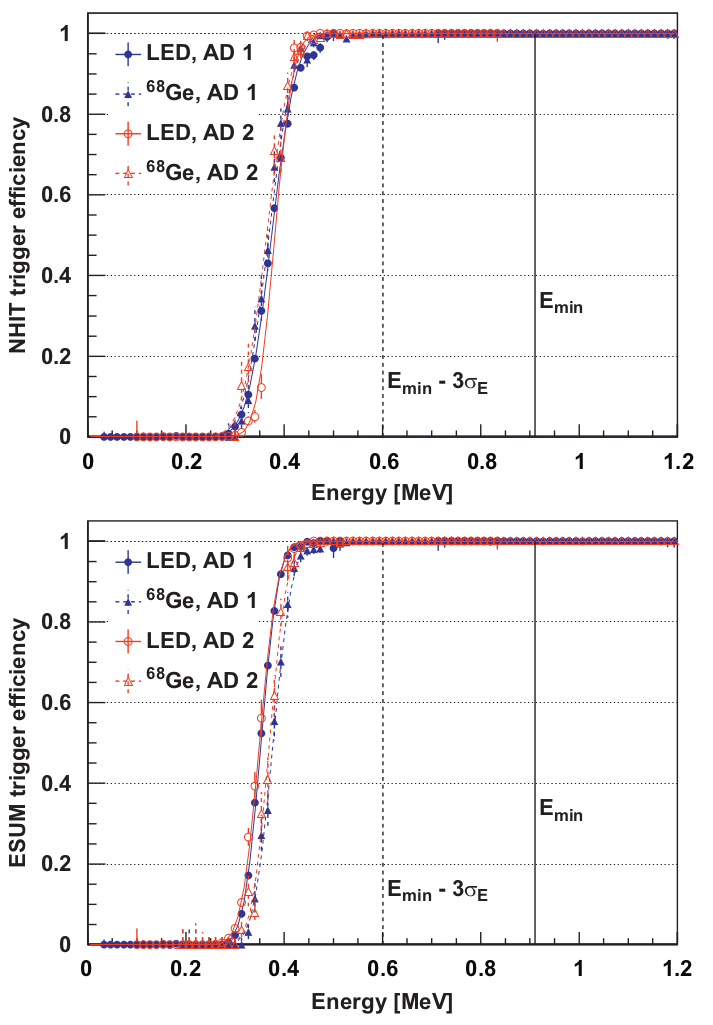
\includegraphics[height=0.8\textheight]{ch_detector/trigger_efficiency_sidebyside}
    \caption{
        Trigger efficiency as a function of reconstructed energy
        at the edge of the AD target volume ($r=\SI{120}{\cm},z=\SI{135}{\cm}$).
        The top figure is for NHIT triggers while the bottom figure is for ESUM triggers.
        Triangles represent efficiency measurements from \isotope[68]{Ge} source data.
        Circles result from LED scans.
        The curves show best fits based on error functions.
        The vertical lines indicate minimum reconstructed energies $E_{\text{min}}$
        of IBD positrons.
        Figure and caption from \cite{sidebyside}.
    }
    \label{fig:trig_eff}
\end{figure}

